%
% Draft  document voiddocker.tex
%
 
\documentclass{article}  % Latex2e
\usepackage{graphicx,lscape,subfigure}
 

\title{Making a docker image to run the Waterfox browser}
\author{Neville Jackson}
\date{4 Sep 2022} 

\begin{document} 

\maketitle      

\section{Introduction} 
This project is about learning how to compose a Dockerfile which runs an X11 application. The Waterfox browser was chosen as an example X11 application, because Waterfox is not available as a package in most Linux distributions, so the result might actually be a useful means of obtaining Waterfox without having to download a tarfile and do a local install. 

Getting a running Docker container to talk to the X11 server in the host system is relatively easy. Waterfox is a large and complex X application, and most of the challenge of this project is in setting up in the Docker image a working environmejnt for Waterfox. 

\section{What is involved in a normal Waterfox install?}
There is a document~\cite{wate:22a} on that.  Briefly the steps are
\begin{enumerate}
\item Download a tarfile from the Waterfox website~\cite{wate:22} or from the Github site~\cite{wate:22b}.
\item  Unpack the tarfile in /usr/local/src
\begin{verbatim}
bzip2 -dc waterfox-G4.1.1.1.en-US.linux-x86_64.tar.bz2 | tar xvf -
\end{verbatim}
\item Make a link in /usr/local/bin to point to the Waterfox binary
\begin{verbatim}
ln /usr/local/src/waterfox/waterfox /usr/local/bin/waterfox
\end{verbatim}
\item Define the desktop icon by adding a file waterfox.desktop to the directory /usr/share applications. The file waterfox.desktop does not come with the tarfile, but is available here~\cite{wate:22a}
\end{enumerate}
We need to implement steps 1 to 3 in a Dockerfile. Step 4 can be omitted, as there will be no icon if running Waterfox in a container. The container will have to be started from the command line.

\section{How to run a docker container requiring access to the host Xserver}
We assume the host is running X11 ( not Wayland ). Set up the following primitive Dockerfile.
\begin{verbatim}
FROM debian
WORKDIR /home/demo
RUN apt-get -y update
RUN apt-get -y upgrade
RUN apt-get -y x11-apps
RUN groupadd -g 1000 demo
RUN useradd -d /home/demo -s /bin/bash -m demo -u 1000 -g 1000
USER demo
ENV HOME /home/demo
CMD /usr/bin/xcalc
\end{verbatim}
 Build this with 
\begin{verbatim}
docker build -t nevj/test:v2 .
Sending build context to Docker daemon  2.048kB
Step 1/10 : FROM debian
 ---> 07d9246c53a6
Step 2/10 : WORKDIR /home/demo
 ---> Running in 2e0e40e0fd4c
..........
Successfully built 517c1937106a
Successfully tagged nevj/test:v2
\end{verbatim}
 Then run it with
\begin{verbatim}
[nevj@trinity dtest]$ xhost +
[nevj@trinity dtest]$ docker run -v /tmp/.X11-unix:/tmp/.X11-unix \
          -e DISPLAY=$DISPLAY -h $HOSTNAME \
          -v $HOME/.Xauthority:/home/nevj/.Xauthority nevj/test:v2
\end{verbatim}
and the xcalc app appears in a separate X window, as shown in Figure~\ref{fig:xcalc}
%\documentclass{article}
%\usepackage{graphicx,subfigure}
%\begin{document}

\begin{figure}[!h]
  \centering
   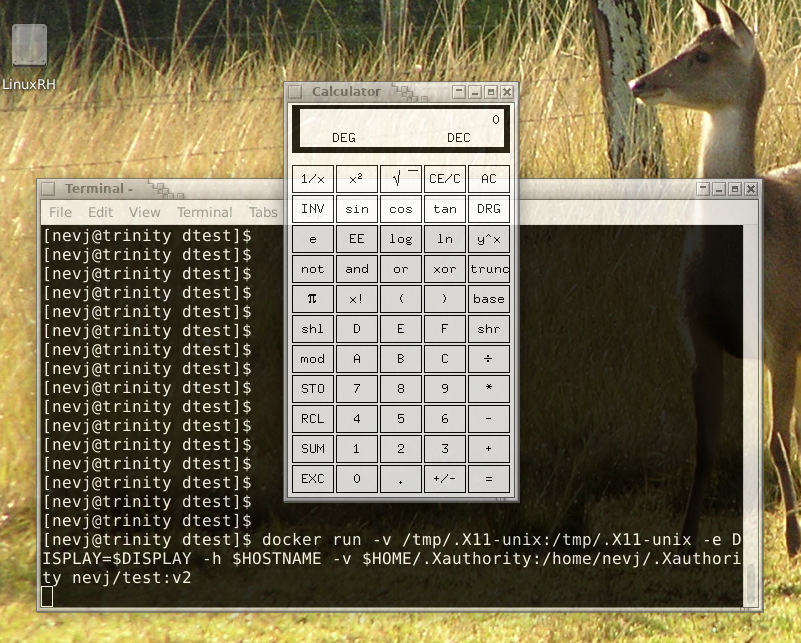
\includegraphics[width=0.9\textwidth]{xcalc.png}
  \caption{Xcalc app started from a Docker container}
  \label{fig:xcalc}
\end{figure}

%\end{document}


The {\em xhost +} statement is needed to give the container permission to communicate with the host X11 server. 
 The purpose of the options included in the {\em docker run} statement are as follows
\begin{description}
\item[-v /tmp/.X11-unix:/tmp/.X11-unix] defines a {\em mount} for a volume. The string {\em /tmp/.X11-unix:/tmp/.X11-unix} is the mount point on the host. The part before {\em ':'} is the volume name on the host. The part after {\em ':'} is where the file or directory is mounted oinside the container. A volume is just a file or directory in the host filesystem.
\item[-e DISPLAY=\$DISPLAY] sets the environment variable DISPLAY in the container
\item[-h \$HOSTNAME] sets the container hostname
\item[\$HOME/.Xauthority:/home/nevj/.Xauthority] sets the .Xauthority file of the container to the .Xauthority file of the host user who initiated the {\em run} statement again using a volume mount.
\item[nevj/test:v2] is the name of te image, build as above.
\end{description}
Volumes are the mechanism used by Docker containers to share data between the host and the container ( and between containers). They are need in this case because the container is an X11 client, while the host acts as the X11 server, so information has to pass between container and host.  A docker container can only write on the part of the host filesystem defined as a docker volume. There is also {\em tmpfs mount} which is a temporary ram disk used for non-permanent data within a container.

\section{First attempt at a Waterfox Dockerfile, using a  Debian parent image}
There is no new principle involved in running Waterfox rather than the simple xcalc app, in a docker container. The Waterfox browser is a large program with many dependencies, so the Dockerfile will have to build up a complete working environment specifically for Waterfox. 

I chose Debian parent image for a first attempt, because Debian is familiar and is most likely to compatable with Waterfox.  The Debian parent image is large. We shall try later to repeat the job with a smaller parent image. 

\subsection{Finding the dependencies of a binary program file}

\begin{thebibliography}{99}

\bibitem{guru:99}
Docker tutorial.
URL https://www.guru99.com/docker-tutorial.html

\bibitem{dock:00}
Docker get started
URL https://docs.docker.com/get-started/

\bibitem{dock:01}
Docker Desktop
URL https://docs.docker.com/desktop/install/linux-install/

\bibitem{dock:02}
Docker Hub
URL https://hub.docker.com/

\bibitem{dock:03}
Official Dockerfile documnet
URL https://docs.docker.com/develop/develop-images/dockerfile\_best-practices/


\bibitem{dock:04}
Dockerfile Guide
URL https://medium.com/@BeNitinAgarwal/best-practices-for-working-with-dockerfil
es-fb2d22b78186

\bibitem{dock:05}
Docker Basics: How to use Dockerfiles
URL https://thenewstack.io/docker-basics-how-to-use-dockerfiles/

\bibitem{dock:06}
A Beginners Guide to Understanding and Building Docker Images
URL https://jfrog.com/knowledge-base/a-beginners-guide-to-understanding-and-building-docker-images/

\bibitem{dock:07}
Best practices for writing Dockerfiles
URL https://docs.docker.com/develop/develop-images/dockerfile\_best-practices/


\bibitem{dock:09}
Creating a Docke Image for your Application
URL https://www.stereolabs.com/docs/docker/creating-your-image/

\bibitem{dock:10}
Docker Containerization Cookbook” - Hot Recipes for Docker Automation
URL https://distrowatch.tradepub.com/free/w\_java39/prgm.cgi?a=1

\bibitem{void:01}
Void Linux Docker Images
URL https://github.com/void-linux/void-docker


\bibitem{libr:22}
LibreWolf source code website.
URL https://gitlab.com/librewolf-community/browser/source


\bibitem{wate:22} 
Waterfox website. URL https://www.waterfox.net

\bibitem{wate:22a}
Install the Waterfox browser on a Linux system. URL https://github.com/nevillejackson/Unix/blob/main/waterfox/waterfox.pdf

\bibitem{wate:22b}
WaterfocCo Github site URL https://github.com/WaterfoxCo/Waterfox/releases

\end{thebibliography}
\end{document}
